\documentclass[../thesis.tex]{subfiles}
\begin{document}

\chapter{Data Management for Devices}\label{sec:data}


\section{Motivation}


Within laboratory research, storage and organization of experimental data is a constant challenge.
Any experiment can generate a large quantity of data in a variety of formats from various instruments.
This data is typically delivered in unlabeled files, with only the name to convey all experimental information.
Further details are left to a lab journal or formal writeup, where researchers outline the experimental procedures and analyze results.
Experimental details and data labeling in this manner is designed to help an active researcher with working knowledge of the experiments understand what has been done.
However, as anyone who has worked in a lab can sympathize with, revisiting work, even your own, after the course of only a few months can often be incomplete, if not enigmatic.
Given these challenges, researchers can often find themselves weighing the benefits of repeating experiments versus finding and attempting to comprehend previous results.

This frustration can be broken into two seperate problem statements.
First, experimental details and data are not intimately connected or collected by default when output from testing equipment.
To find results, often experiments have to be searched for in a lab notebook, then cross referenced with electronic files.  
This relies on the searcher paging through notebooks, interpretting scribbled notes that were made, and hoping that whatever title was chosen for the days experiment to obviously identify what they are looking for.
Then, assuming at best that this researcher provided a full filepath to experimental data on a computer that doesn't exist in your lab anymore, you have the task of searching through poorly labeled folders on a backup drive somewhere to find the data.
As a researcher, it is nearly impossible to make this foolproof for later use, especially in an academic setting, since these is no standardization of storage location or note taking applications.
Corperate research facilities often use electronic lab notebooks and project archives to help have collected digital archives to mitigate this problem. 

The second issue is the exclusion of critical information.  
In any experiment, there are numerous experimental parameters and details that need to be recorded. 
It can be easy to dismiss details as obvious or commit to memory for the purpose of analysis, then omitting this from the written information.
However, when revisiting the experiment, these details are rarely obvious.
An example out of this in our lab, is the planarizing layer in devices for lifetime testing.
For large area patterned devices, we always use a planarizing layer, and for almost two years, that was always PEDOT-PSS.
With this the case, it was considered almost a part of the substrate, and could be excluded from experimental details as it was implied.
However, over time, we transitioned to using Plexcore AQ-1200, and then to AQ-1250 when AQ-1200 was discontinued.
This easy and obvious case rapidly turned into a complex history, which could not have been predicted.
The simple answer to this is to record every experimental parameter, but this is not logistically possible.
Often it is even difficult to assess what is a constant and what will change.

While it can be easy to dismiss these issues as a problem for individual researchers, it is important to acknowledge that these are systematic issues and it should be a collective goal to minimize these issues.
Every researcher attempts to provide clarity in this messy system, but the truth is that organizing and collecting data well using this system takes valuable time and effort that is hard to allocate and is not often appreciated until much later.
Proposed methods for addressing these issues have to combat workflow inertia, and the resistance to change.
Ideally, solutions will not interfere were current methods, and will make work easier in the active workflow as well as in archive searching.

\begin{wrapfigure}{r}{.5\textwidth}
\centering
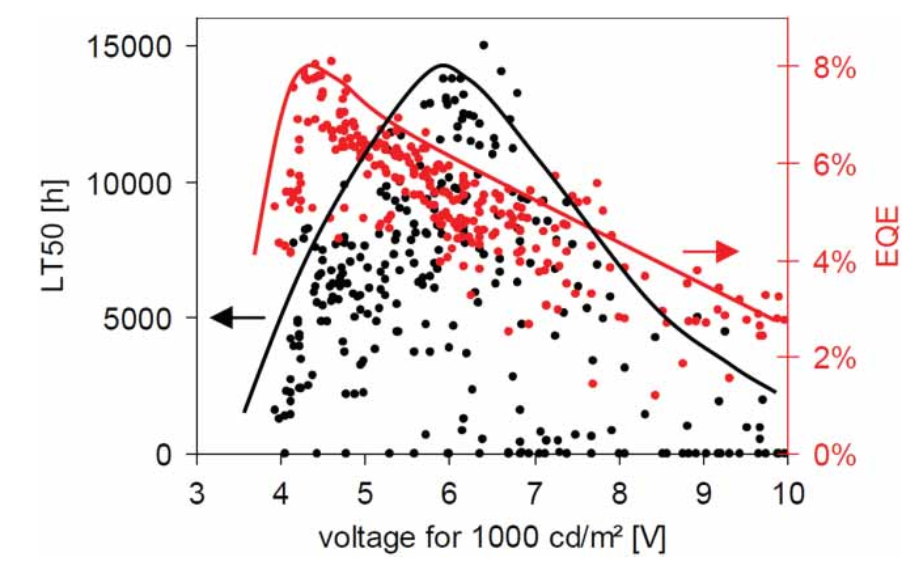
\includegraphics[width=.5\textwidth]{data/bohm}
\caption{Dependence of EQE (red) and lifetime (black) on the driving voltage for various ETL configurations, sharing same HTL and EML. Reproduced from \textcite{Bohm2011}.}
\label{fig:bohm}
\end{wrapfigure}

Commercially, this issue of keeping track of experimental data is largely resolved.
This is due to an ability to mandate research standards and organization required at this higher throughput scale.
While the methods are not published, an example of commercial data management is shown from Merck \& Company, Inc. in Figure \ref{fig:bohm}.
This figure references hundreds of efficiencies and lifetimes with extracted peak EQE characteristics and operating conditions.
Without data management, figures and conclusions like this would not be possible to make.

Within our lab, I have made an effort to address these issues using a relational database.
This collects all data and connects with experimental details, and allows for easy search and manipulation of data in a standardized format.
The details of implementation and usage examples are provided in this Chapter.

\section{Overview}

The first issue addressed above is the seperation of experimental details from the actual collected data.  
This is almost universally resolved using relational databases.
In a relational database, a series of records are stored with a list of attributes and values.
Individual records can be looked at and all of the information is well organized.
However, this system becomes increasingly valuable if records share a list of attributes, where the records can be searched based on the values of certain attributes.

Relational database systems are largely catagorized into SQL and non-SQL systems.
In SQL, all data is organized into tables, providing a relatively rigid structure.
If values are not single valued, it is often necessary to create additional tables.
Without going into further detail, non-SQL database systems are more ideal for laboratory data, as they have better support for list form values.
With this in mind, I have developed this data collection system using MongoDB, a widely accepted non-SQL database.
Mongo supports interfacing directly as well as multiple other programming languages, including Python, the language I have utilized.

To facilitate this discussion, a few terms need to be defined.  
In the world of Mongo, a "Document" is a single entry of data with many keys (attributes) and values, equivalent to a record in SQL.
An example of this is:

\begin{lstlisting}
{
        Name: Kyle Hershey,
        Occupation: Researcher,
        Lab: 421,
        Location: Minnesota
}
\end{lstlisting}

Here, several pieces of connected information are collected, creating a document.
In this example, "Name" is a key, while "Kyle Hershey" is the associated value.
Every document stored in Mongo also has a unique ID, that can be used to reference it.
Several Documents sharing the same type of information are organized into a "Collection".
A Collection of Documents like the one above would serve as a sort of directory of people.
In Mongo, not all Documents in a Collection are required to share the same list of keys.  
For example, other Documents may add a "Phone Number" or exclude the "Lab".
However, Collections are intended to provide Documents with common information.
A "Database" is a series of Collections that have related in formation and interact with each other.
For example, a seperate Collection in the same Database may store information about every lab.


\begin{lstlisting}
{% Database 
    {% Collection : People
        {% Document
            Name: Kyle Hershey,
            Occupation: Researcher,
            Lab: 421,
            Location: Minnesota
        }
        {% Document
            Name: Russell Holmes,
            Occupation: Professor,
            Location: Minnesota
        }
    }

    {% Collection : Labs
        {% Document
            Lab: 421,
            Function: OLED deposition,
            PI: Russell Holmes
        }
    }
}

\end{lstlisting}

This would then be able to be cross-referenced between the Collections for further information.
If a value referencing another collection is not unique to a single document, the Document ID can be used.


\section{Organization}

As mentioned previously, databases require consistency of documents within the collection.
This can be difficult to do effectively within a research environment where experimental design can change frequently.
Within our lab, I have capitalized on the workflow of our experiments in order to organize the collections.
The four primary collections for daily workflow are \textbf{materials}, \textbf{architectures}, \textbf{growths}, and \textbf{lifetimes}.
A full list of keys and datatype expectations can be found on the wiki page at \url{https://github.umn.edu/HolmesGroup/lifetimeTesting/wiki}.

At the most basic level, any film or device consists of a series of materials that are utilized for their physical properties.
The \textbf{materials} collection seeks to keep track of all materials used in our lab and their various properties.  
Most notably, this includes energy levels, differing names, the CAS number, melting temperature and glass transition temperature ($T_g$).
The other collections in the database utilize the material ID from this collection to uniquely identify materials for searchability and cross-referencing purposes.

The \textbf{architectures} collection captures the information required to describe what is grown.
This includes the materialID (from the \textbf{materials} collection) and thickness for all substrate and deposited layers.  
Additionally, standard information like the EML thickness, doping concentration, and architecture type are stored for easy lookup.

For a planned experiment, once an architecture is decided upon, the experiment needs to be executed.
An individual object in the \textbf{growth} collection consists of a single device architecture and the characterization data associated with the set.
Characterization data includes all steady-state, standard characterization measurements, including spectrums, \eqe, power efficiency,  and current-voltage-luminace characteristics, among others.
All data is stored for every device pixel, and is labeled by substrate and pixel number.
Additional data about the experiment including the date, last chamber clean, grower name, and additional notes and reference tags is also collected.

Frequently in my work, in addition to steady state measurements, the operational lifetime is characterized.
The \textbf{lifetimes} collection stores all information about lifetime measurements.
This includes operating conditions, the associated \textbf{growth} and \textbf{architecture}, performance as a function of time, as well as any additional notes.
Lifetimes are connected to the individual pixels from a \textbf{growth}.

This hierarchy creates lifetime objects which stems from a single growth, stemming from a single architecture.  
However, an architecture can be the base of multiple growths, which can each have multiple lifetimes.  

Various spectral characterizations are stored in seperate collections.  These include photoluminescence, absorption, and excitation spectra, as well as optical constants.
Each of these collections stores a layer structure, relevant illumination and testing conditions, tester name and date, as well as other test information.

\section{Applications}

Using this organizational framework for our data, I wanted to make sure all test information was recorded in this format to ensure utilization.
In order to do this, I thought it was important to minimize the energy barrier for usage, and integrate usage of the database into the daily workflow.
Since implementation, the database is now a critical part of data collection and analysis for OLED characterization in our lab, even offering new features that were not possible before.
This section seeks to outline some of the key areas of use and capabilities of this database system.

\subsection{Growth Characterization}

After a growth is completed, spectral and current voltage characterization needs to be done.
All of this data collection is done on a laboratory computer.
Previously, generated datafiles would be transfered using a flashdrive to the researcher's computer, where they would be organized and analyzed.

\begin{figure}[ht]
\centering
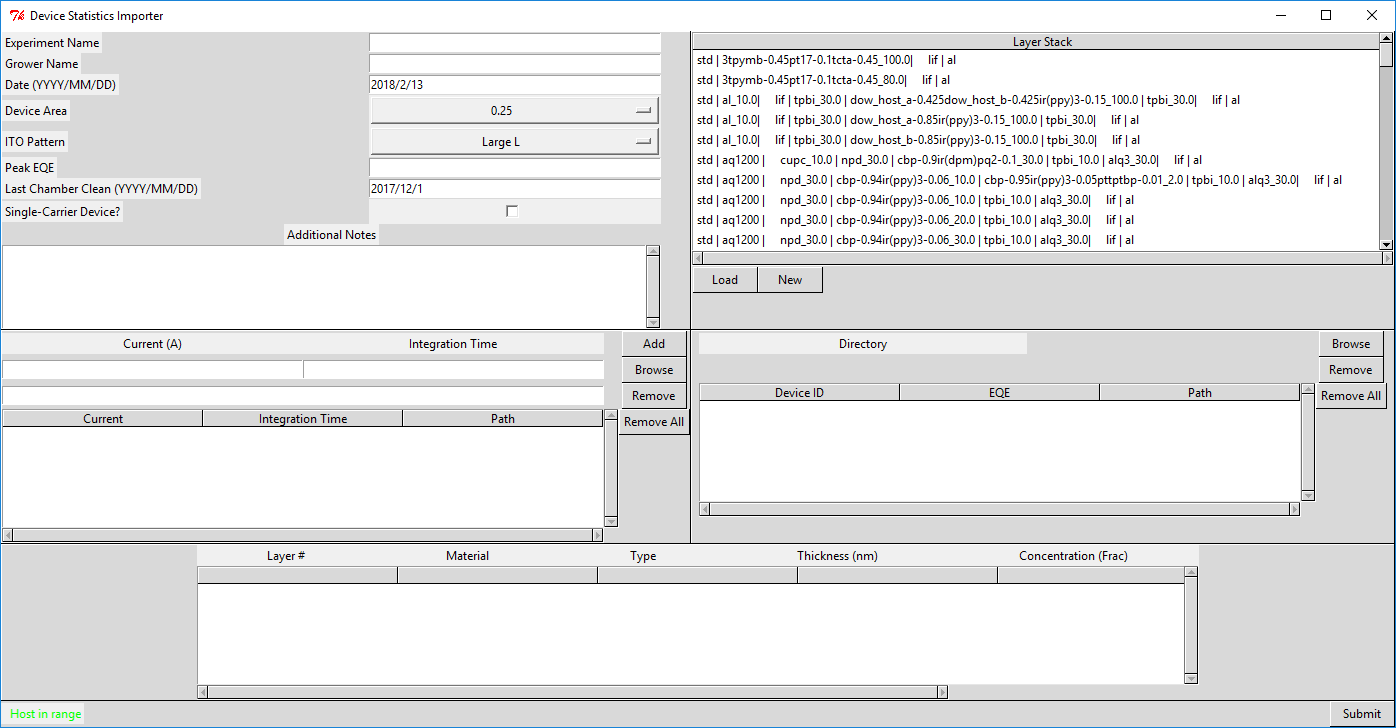
\includegraphics[width=\textwidth]{data/growthStats}
\caption{Graphical Interface for uploading test data into the database.}
\label{fig:growthStats}
\end{figure}

I developed a Graphical User Interface (GUI), shown in Figure \ref{fig:growthStats}, in order to collect all of the test information into the database.
In the top left panel of Figure \ref{fig:growthStats}, basic test information can be entered.  
The top left allows selection of the architecture that was grown, or creation of a new architecture.
Once loaded, the layer stack of the selected architecture will be displayed in the bottom panel of the interface.
Spectral data can be input in the middle left panel, with current and integration time automatically extracted from the filename.
Current-voltage characteristics can be selected using the middle right panel, with the substrate and device number extracted from the filename.

Once completed, this form can be submitted and the information will be entered into the database.
Before submission, the entered data is analyzed, and the \eqe, luminance, power efficiency, as well as numerous other calculations are performed and stored along with the raw data.
This reduces the workload of the researcher because they no longer have to do the analysis or transfer the files manually.
Plotting the calculated data is the only task remaining for the user.

Two primary workflows have been developed for plotting and comparison of test data.  
For publication quality figures, our group historically has used Origin.  
To implement this, I developed another interface, shown in Figure \ref{fig:idSelector}.
This interface allows easy selection of datasets either by growth or architecture.
Once the data sets are selected, the desired plots are selected and the data is sent to origin where polished plots and worksheets are created.

\begin{figure}[ht]
\centering
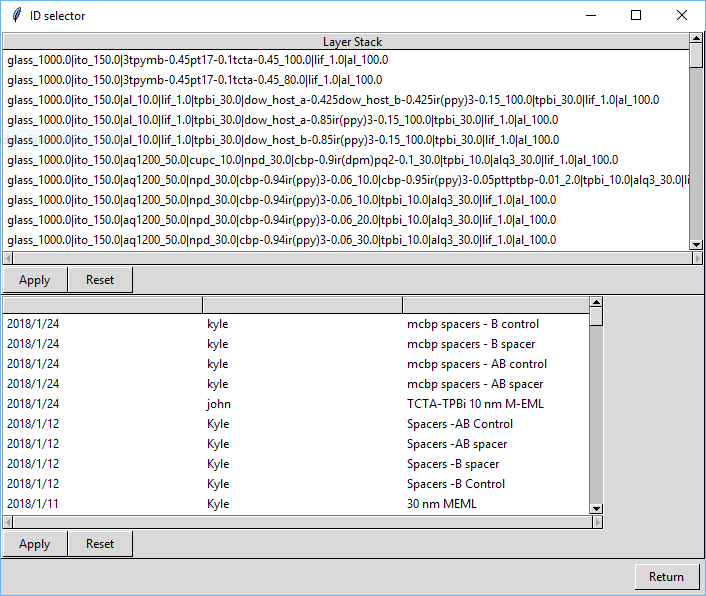
\includegraphics[width=\textwidth]{data/idSelector}
\caption{Graphical Interface for selecting data to send to Origin.}
\label{fig:idSelector}
\end{figure}

Within the database, representative IV scans can be identified by editing the \textbf{trust} key.
The Origin plotter will not plot scans with a low trust factor, but will import the worksheet.
This makes it easy to compare datasets without having to first remove bad scans.

This GUI is useful as it fully replaces the previous behavior of manual file transfer and analysis, but adds on the ability of being able to easily access and compare any previous datasets.
This selection process is efficient for standard characterization and processing, but is not very flexible when it comes to non-standard analysis or more intricate data selection.

Given the advanced sorting and organizational possibilities of the database, it is easy to select different data based off of criteria that the interface shown in Figure \ref{fig:idSelector} does not allow.
For example, what if we wanted to know to compare devices that used the material TCTA and had an EML thickness of 30 nm?
This can be trivially done in python using the following command:
\begin{lstlisting}
{
    selectedArchitectures=db.architectures.find({'eml_thickness':30, 'layers_list.material': 'tcta' })
}
\end{lstlisting}

With this ease of selecting data, a flexible plotting solution is needed to accomodate analysis or the resulting data.  
Primarily, we have settled on using Python in Jupyter Notebooks with Matplotlib for plotting.
This allows for easy data selection, programatic analysis, and plotting, all in a well organized notebook-like format.

\begin{figure}[ht]
\centering
    \begin{subfigure}{.4\textwidth}
    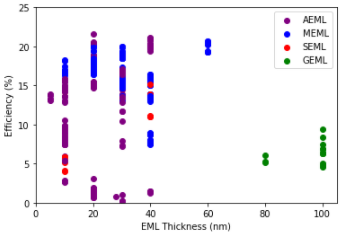
\includegraphics[width=\textwidth]{data/growthDBexamples2}
    \caption{}
    \label{fig:growthDBexamples1}\par\vfill
    \end{subfigure}
    \begin{subfigure}{.4\textwidth}
    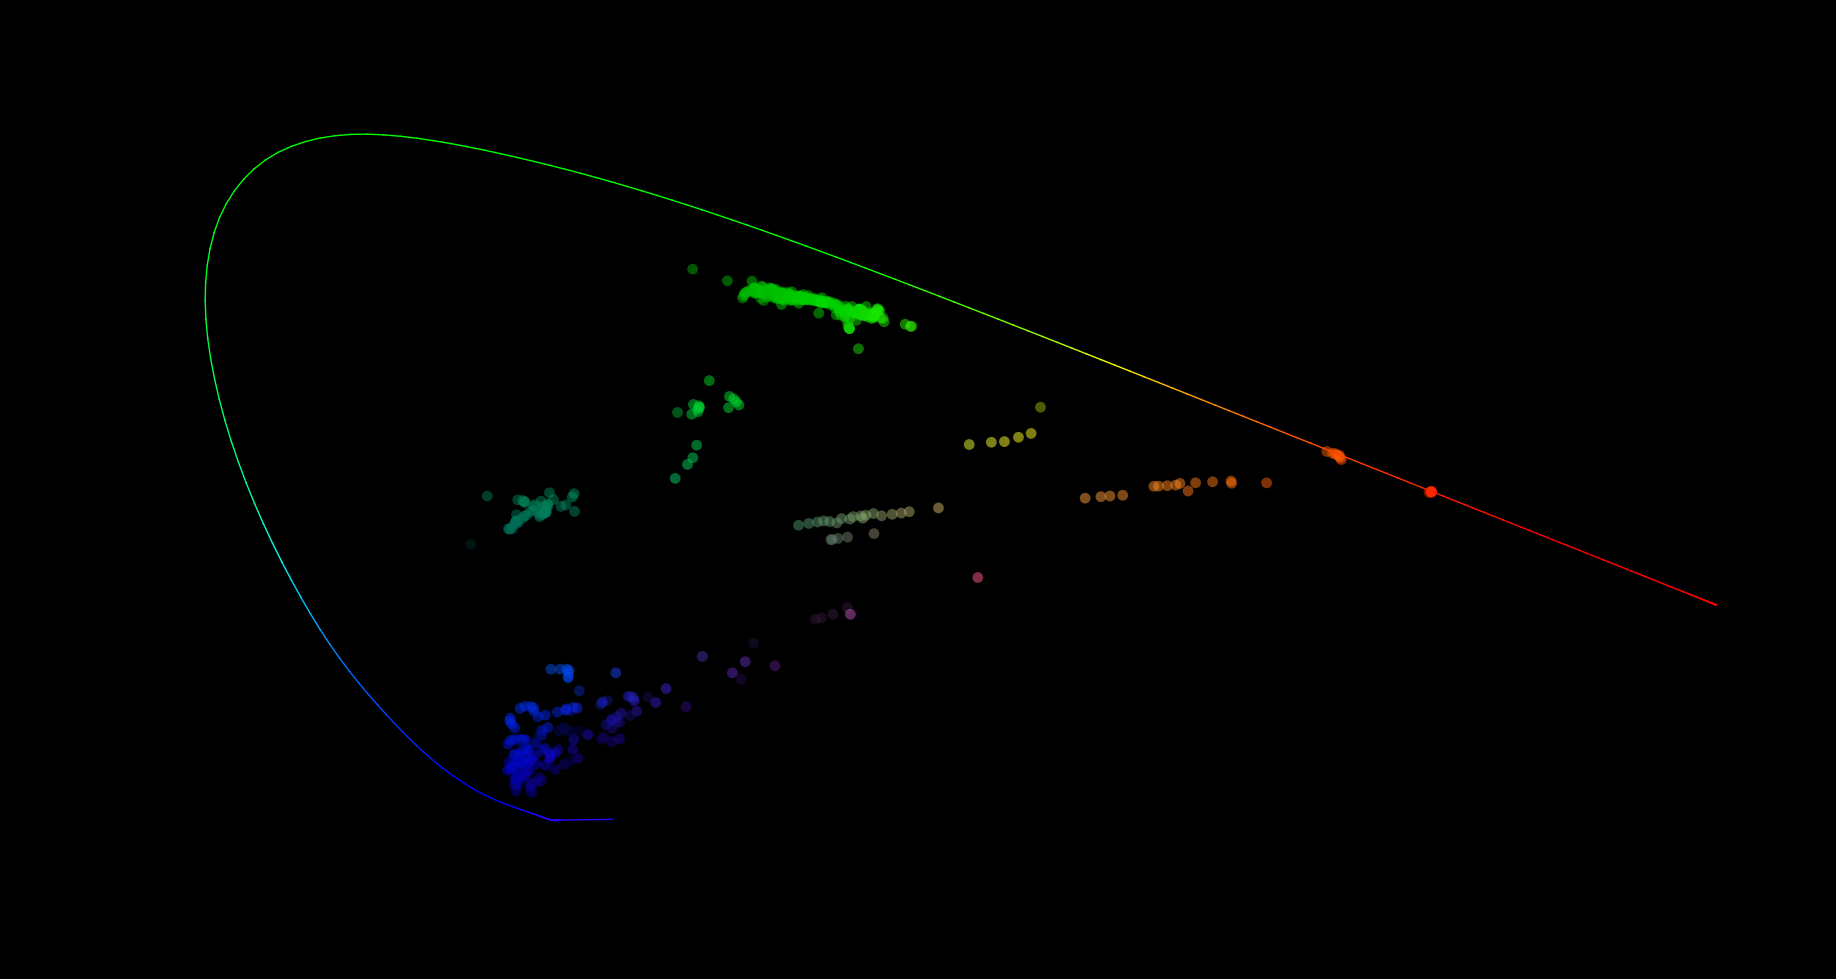
\includegraphics[width=\textwidth]{data/cie}
    \caption{}
    \label{fig:data_cie}\par\vfill
    \end{subfigure}
\caption{  a. Peak EQE as a function of EML thickness b. CIE coordinates of every device collected during my thesis. }
\end{figure}

The first example, shown in Figure \ref{fig:growthDBexamples1}, investigates the overall behavior of \eqe as a function of the EML thickness for various device types.
This was obtained using the following segment of code:

\begin{lstlisting}
{
    growths=db.growths.find({,{'architectureID':1,'devices.peakEQE':1,'devices.trust':1})
        colors={'MEML':'blue','AEML':'purple','SEML':'red','DEML':'orange','GEML':'green'}
        for growth in growths:
            arch=db.architectures.find_one({'_id':growth['architectureID']})
            nm=arch['eml_thickness']
            color=colors[arch['device_type']]
            for device in growth['devices']:
                if device['trust']>1:
                    plt.scatter(nm,device['peakEQE'],label=arch['device_type'],c=color)
    plt.legend()
    plt.show()
}
\end{lstlisting}

This search accesses a variety of information about almost 200 growths over the last 5 years.
This plot consists of thousands of reference points, which are all easily organized due to the database.

It is also important to note that further analysis can be conducted after data selection, as well as plotting.
A good example of this is shown in Figure \ref{fig:data_cie}.
This figure shows every device spectra that I have collected during this thesis, with CIE color coordinates calculated for every spectra.

These examples are not included for interest in the data itself, but for the ease of comparison and compilation.
Without the database, organizing these datasets would be a nightmare of digging through lab notebooks and computer files, followed by a painful graphing process with dozens of files.
The energy barrier of compiling this data would be enough to deter most researchers from even attempting to look for trends like this.

\subsection{Lifetime Characterization}

After devices are grown and characterized, they are immediately entered into the database.  
The lifetime testing setup capitalizes on this and connects the lifetime test data to the growth on startup.
After hitting start on a lifetime test, the interface shown in Figure \ref{fig:dbImporter} must be filled out before the test will start.  
The test automatically populates the testing conditions, and the user is able to add additional information.
The menu in the top left allows easy selection of a growth to connect to.  
If a luminance is entered here, the current can be calculated for operation based off of the IV scan for the exact device being tested.
This eliminates a loading step of having to measure the luminance again with a luminance scope.
Since this menu is part of the user experience of loading lifetimes, all lifetimes are seemlessly logged.


\begin{figure}[ht]
\centering
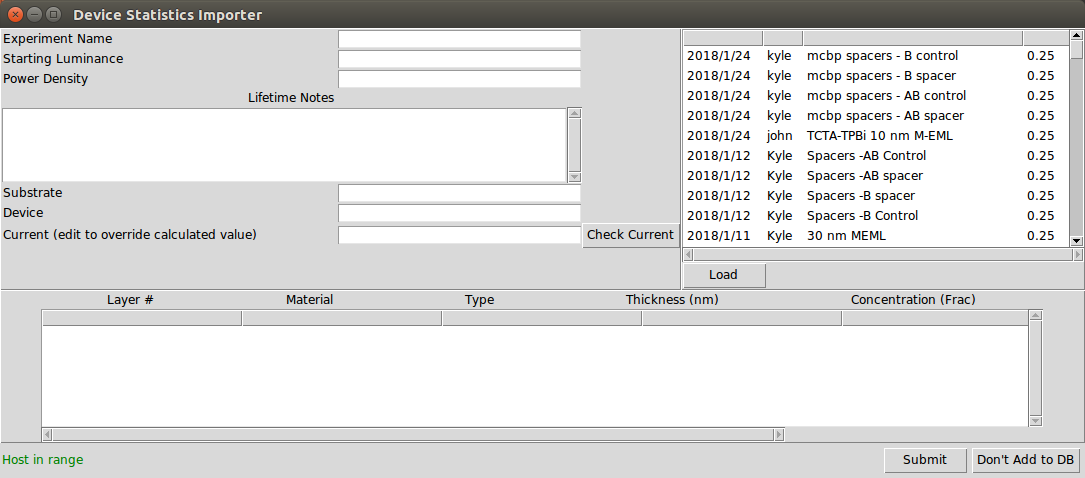
\includegraphics[width=\textwidth]{data/dbImporter}
\caption{Graphical Interface for importling lifetime to database.}
\label{fig:dbImporter}
\end{figure}

As the test is running, data is actively uploaded to the database, rather than waiting for the end of the test.
A jupyter notebook interface has been developed to plot all actively running tests.
This allows remote monitoring of all running lifetime tests distributing between the four lifetime testing platforms in our labs.
Upon test completion, the user gets an email alert that the test has completed, along with a graph of the lifetime results.


\begin{wrapfigure}{r}{.5\textwidth}
\centering
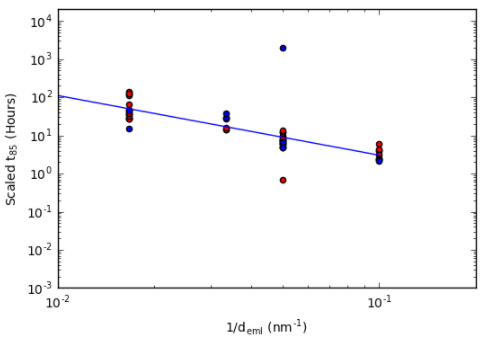
\includegraphics[width=.5\textwidth]{data/growthDBexamples3}
\caption{Device lifetime for a particular set of devices as a function of EML thickness. All lifetimes scaled to 3000 cd/m$^2$, with scaled lifetimes shown in red.}
\label{fig:data_meml}
\end{wrapfigure}

Similar to the growth collection capabilities, the lifetime collection allows unique filtering and analysis capabilities.
A practical application example is from the work in Chapter \ref{sec:lifetime_meml}.
In this work, a relation is shown between the exciton density and the device lifetime.
The exciton density can be manipulated using the EML thickness.
In this system, the scaling function of lifetime as a function of luminance is known.  
Looking at all devices using a TCTA:TPBi MEML structure with 5\% doping and scaling all lifetimes to 3000 cd/m$^2$, a relationship is seen between $d_{EML}$ and the device lifetime, as shown in Figure \ref{fig:data_meml}.
In fact, a scaling relation can be extracted, similar to the one shown for luminance.
Prior to the completion of the dataset, we had hypothesized that this relationship existed.  
By utilizing these capabilities of the database, we were able to observe this relationship, further motivating the completion of a constant luminance dataset, which is shown in the final work.


\subsection{Materials Properties}

The Growth and Lifetime collections offer a lot of features that are useful for device fabrication and characterization.
The materials and spectral collections help in providing a well organized collection of materials characteristics.
The simplest example of this would be a list of all known energy levels of materials, as shown in Figure \ref{fig:data_mats_By_homo}.
This dataset is actually much more rich than it first may appear.  
For a given material, multiple values can be stored, along with their literature reference.
An accepted value can be identified as well.

\begin{figure}[ht]
\centering
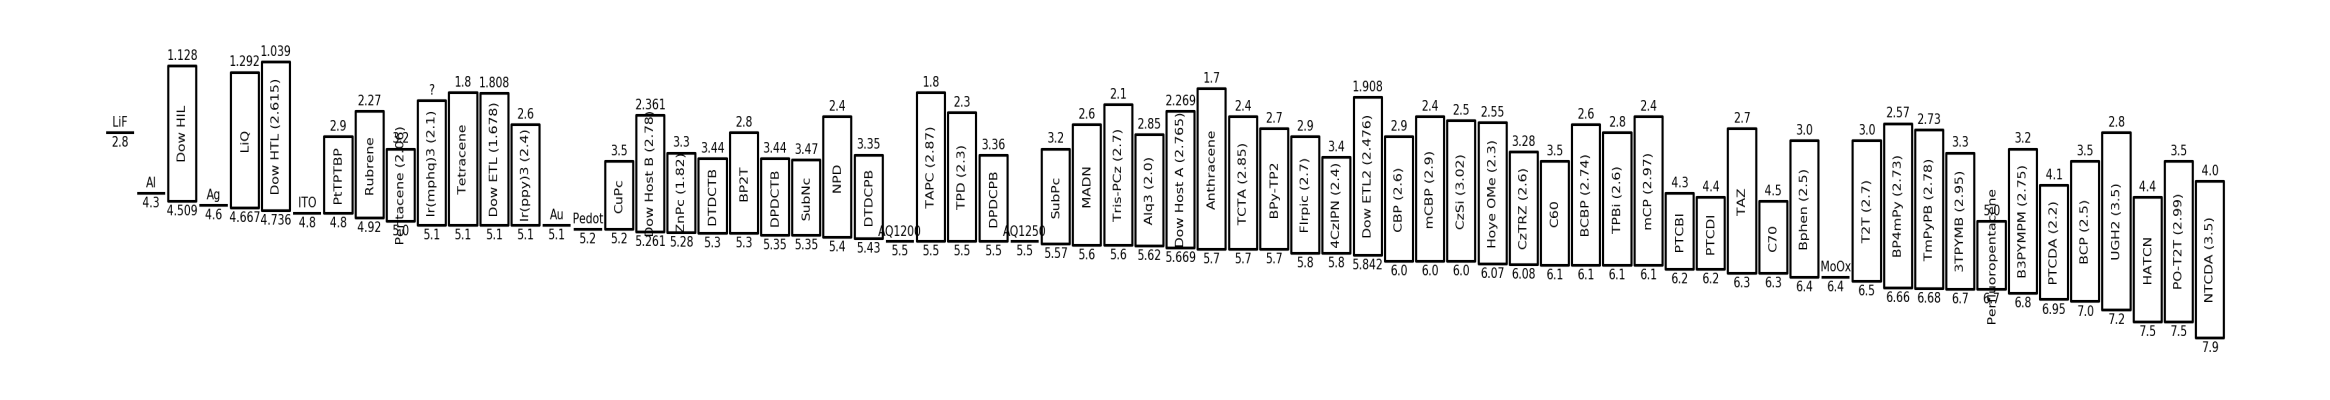
\includegraphics[width=\textwidth]{data/mats_by_homo}
\caption{Energy levels of materials in database, sorted by HOMO value.}
\label{fig:data_mats_By_homo}
\end{figure}

Spectral data can also be very important in material analysis.  
I have collected a large number of spectra recorded from the fluorimeter and UV-Vis, to populate the plSpectra, absSpectra, and excitaionSpectra collections.
These collections can be easily search by material name and spectra type, using the Jupyter Notebook available at \url{http://holmes-carl.cems.umn.edu:8888/notebooks/databaseNotebooks/Spectra\%20-\%20Search\%20.ipynb}.
This notebook plots all spectra for the selected material, allowing variation and average features to be seen.


\begin{figure}[ht]
\centering
    \begin{subfigure}{.4\textwidth}
    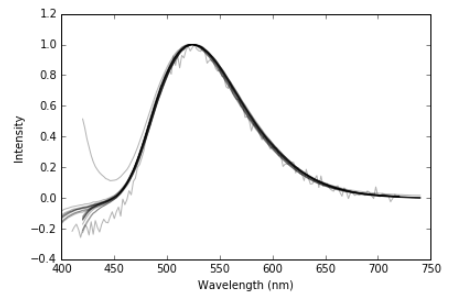
\includegraphics[width=\textwidth]{data/alqSpectra}
    \caption{}
    \label{fig:data_alq}\par\vfill
    \end{subfigure}
    \begin{subfigure}{.4\textwidth}
    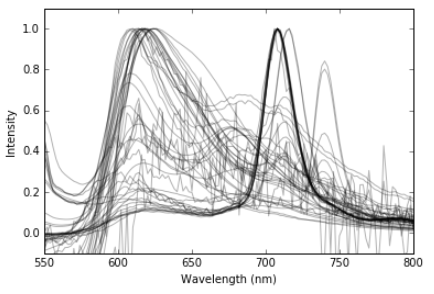
\includegraphics[width=\textwidth]{data/subpcSpectra}
    \caption{}
    \label{fig:data_subpc}\par\vfill
    \end{subfigure}
\caption{  a. All collected spectra for Alq$_3$.  b. All collected spectra for SubPc.}
\end{figure}

Example output of this utility program can be seen in Figures \ref{fig:data_alq} and \ref{fig:data_subpc}.
For Alq$_3$ in Figure \ref{fig:data_alq}, very consistent emission is seen, representing an efficient, well behaved emitter.
However, Figure \ref{fig:data_subpc} shows the spectra for SubPc, a weak emitter that has been problematic in our group in that different batches and processing conditions can show varying spectral behavior.
Two clear spectral features are shown as the most dominant, though they vary dramatically in intensity.
Previous efforts to understand the changing spectra have relied on lab notebook notes and memory to understand differences between the spectra, and have been largely unsuccessful.
Hopefully, with improved recording of parameters using the database for future tests, a more complete understanding can be obtained.

Our group does a large amount of optical field modeling for layer stacks that relies upon optical constants obtained by the group.
Standard procedure for management of these optical constants has been to share an excel document with obtained constants to new students, and selectively distribute new measurements as needed.
This has resulted and every researcher having a differing set of constants and often various files with incomplete sets.
Additionally, no experimental details are included, other than the results, making the history and validity of constants always being a problem.

With optical constants being included in the database, a central repository of constants has been developed, that can include all relevant test information for the curious researcher to use as needed.
Developed by my collegue John S. Bangsund, a Transfer Matrix simulation package is now available to the group at \url{https://github.umn.edu/HolmesGroup/holmesPackage}.
This package is capable of doing most Transfer Matrix calculations while fetching all necessary optical constants from the database.
This eliminates any need for individual collections and makes any new data instantly available to the whole group.

\subsection{Available Programs}

In developing a workflow around using this database for data collection and analysis, John S. Bangsund and I have created several useful programs utilizing database features.
These are available internally within the UMN at \url{http://holmes-carl.cems.umn.edu:8888/tree/databaseNotebooks}.
A brief summary of useful programs is provided below.

\begin{itemize}
\item \textbf{Daily Analysis:} Allows selection of growth and plots all related IV, \eqe, and lifetime plots.  Serves as a template for analysis of a growth.
\item \textbf{Database Query Examples:} A guide for building queries to find tests.
\item \textbf{Energy Level Diagrams:} Constructs an energy level diagram that can be downloaded as an image.  Energy levels are obtained from the materials collection.  Diagrams can be constructed from a selected architecture, or from a custom list of materials.
\item \textbf{EQEtrustAsses:} Allows selection of representative \eqe scans for a growth.
\item \textbf{lifetimeTrustAsses:} Sets the validity of lifetimes connected to a growth or architecture.
\item \textbf{plotCurrentLifetimes:} Plots all actively running lifetimes in all boxes.
\item \textbf{plotRecentLifetimes:} Plots lifetimes run recently.  Date range is selectable.
\item \textbf{Spectra - Search:} Advanced search tool for various spectral characterizations.
\item \textbf{Tooling Factors:} Allows plotting of tracked tooling factors over time and as a function of deposition rate.
\item \textbf{Importers (Folder):} Import functions for spectra into the database.


\end{itemize}

\section{Future}

The usage of a database system for organizing laboratory results for OLEDs have dramatically changed our workflow for the better.
Data is easily and perminantly logged in a format that is easily searchable and programatically accessible.
This has provided multiple capabilities that we did not previously have.
Implementing this system to the point it is today has required significant investment of time and energy without generating immediate forward research progress.
This has included thousands of lines of code and over 350 versions of the front-end software.

Thankfully, our team of OLED researchers has found this investment to be very useful and we have fully commited to using this system.
All aspects of growth, materials analysis, lifetime and steady-state characterization are recorded and analyzed using this system.
These analyses are standard procedures for our lab and invariant with time, providing consistent data compatible with a research database.

We have found that there are some experiments where the database system is not advantagious.
For this system to be useful, a standard data structure is needed to provide easy searching and extraction of data.  
Often, for one time, novel experiments, there is minimal overlap with other tests.  
In these cases, logging experiments into the database does not fit the structure of other documents, and trying to force compliance into this system is not worth the effort.
An example of this is optical degradation, where currently, no standard procedure has been developed.
In these cases, it is difficult to identify important test parameters to record, and often results are not comparable even if they were recorded.
In these cases, experimental methods need to develop sufficiently before logging into the database becomes useful.
Moving forward for OLED research, it will be important to identify where this system can provide utility, and where it may not be worth the effort.
Additionally, recognizing when new experiments have reached sufficient maturity to be worth archiving will require active dialogue.
However, given the value that this database archive has provided, I have confidence that it will continue to be used and expanded.

\subsection{Machine Learning}

Having a well populated dataset such as this also opens up the possibility for use of machine learning algorithms.
Machine learning uses a large dataset to train an algorithm which in turn will predict outcomes of future data into either catagorical or numerical output.
With enough examples that have all input variables, the algorithm can predict many different behaviors.
Due to the complexity of OLED design, and number of unknown variables, predicting \eqe or lifetime from material information is unrealistic.
However, less complex problems are solvable and can offer insight and utility into the manufacturing of devices.
Here, I will outline three ventures into this space that I have conducted initial attempts to aid in research.


\begin{figure}[ht]
\centering
    \begin{subfigure}{.3\textwidth}
    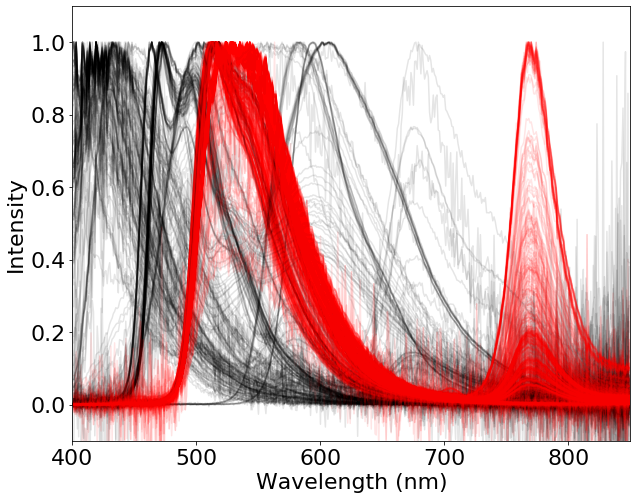
\includegraphics[width=\textwidth]{data/irppyLearn}
    \caption{}
    \label{fig:data_ml_irppy}\par\vfill
    \end{subfigure}
    \begin{subfigure}{.3\textwidth}
    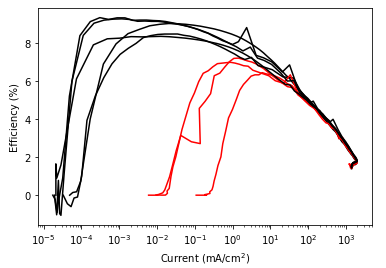
\includegraphics[width=\textwidth]{data/trustLearn}
    \caption{}
    \label{fig:data_ml_trust}\par\vfill
    \end{subfigure}
    \begin{subfigure}{.3\textwidth}
    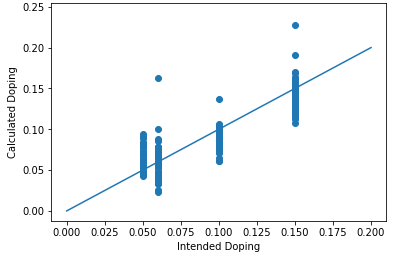
\includegraphics[width=\textwidth]{data/concentrationLearn}
    \caption{}
    \label{fig:data_ml_concentration}\par\vfill
    \end{subfigure}
\caption{  a. Machine learning to spectrally identify Ir(ppy)$_3$.  Spectra shown in red are identified by the program as containing Ir(ppy)$_3$. b. Identifying and removing bad \eqe scans.  Spectra shown in red are identified as not representative and bad.  c. Predicting concentration base on spectra.}
\end{figure}

The first application is in predicting the emissive molecule from a PL spectra.
Initial attempts at this involved identifying Ir(ppy)$_3$ emission, shown in Figure \ref{fig:data_ml_irppy}.
In this figure, the \irppy feature is successfully identified, and depending on the algorithm training, can be taught to include or exclude the devices featuring the PtTPTBP sensitizer, whose emission is seen at 780 nm.
While identifying the most recognizable emission feature from our lab is not very useful, this type of training could be useful for identifying unrecognized features.
For example, if an impurity is seen in emission, it may be from a more exotic molecule.  
By having a trained algorithm to identify the emission, the researcher could be saved from having to look through spectra from every molecule.
This identification could be done using a catagorical algorithm.
The implementation of a full identifier that can recognize all molecules has been hindered by the lack of spectral data for some molecules.
The ability to predict output depends heavily on the size of the training set, so it is important to have a large number of example spectra.
As more data is uploaded from the group, the resolution of this program will improve.

The second example is to identify bad IV scans, shown in Figure \ref{fig:data_ml_trust}.
This was an attempt to identify features of good \eqe scans, using all devices in the database as a reference.
However, this study found that given that all devices are not ideal, representative ``good'' behavior is not consistent between devices.
Therefore, the ability to recognize characteristic behavior for all devices is variable.
While the example in Figure \ref{fig:data_ml_irrpy} shows reasonable seperation, there are other device sets that predict that all devices are bad.
For better results, identified good and bad devices from the same architecture should be used.
An interesting application of this would be to store trained algorithms for each architecture within the database, providing much better catagorization.
Then, when a new stack is grown for an existing architecture, the algorithm could identify scans immediately upon upload.
Given the variety of devices we tend to grow, this would not be useful for most cases, but might be for benchmark devices.

The third application is an attempt to spectrally identify the Ir(ppy)$_3$ concentration.
This algorithm takes in the device spectra and predicts the \irppy concentration.
Figure \ref{fig:data_ml_concentration} compares the intended and predicted concentration, and surpringly shows a reasonable correlation.
The astute reader would note that the emission should also be a function of the emitter distance from the metal interface.
However, further attempts at improving this algorithm are mostly limited by knowledge of the actual variation in the intended concentration.
Since the reference value has a relatively large error bar, the accuracy of the training set is relatively low and limits the ability to resolve concentration differences.

These examples do not represent the full capabilities of machine learning, but offer some ideas as to useful information that it may provide.
Given the amount of data that is being generated and input, it is important to think of applications for machine learning to help improve and provide feedback that will help the researcher.  
Abilities of this setup, especially with regards to spectra characterization, will greatly improve if a larger portion of the group begins to utilize the capabilities of the database.


\subsection{Extension to Solar Cells}

Given the success and utility of this database for OLEDs, an obvious extension in our group is the application to solar cells.
Solar cells share much of the same data format to OLEDs: Materials are characterized in the same way, architectures and growths are conducted in the same manner with the same equipment, and characterization shares many similarities.
Minimal modification of current analysis and plotting scripts is needed to start collecting solar cell research data into a similar system.

Despite the advantages and currently developed code base, a solar cell research database has yet to be utilized within our group.
This has largely been due to resistance to a change in workflow.
Most data analysis within the solar cell research in our group is done within Matlab, with test data loaded from files.
MongoDB does not have a Matlab driver, and for OLEDs, we have developed our scripts in Python.
For established researchers, transitioning existing workflow and learning a new programming language is seen to outway the advantaqes of the database system.
In order for the database to be utilized, new students will have to develop the analysis workflow to help establish this technique for solar cells.

\subsection{Perovskite Film Growth}

While vacuum-deposited solar cells share many similarities to OLEDs and the existing data, perovskites offer unique challenges to organization.
For vacuum deposited OLEDs with reproducible growths, the discussed data structre allows for easy comparison against architectures, and growths should be relatively consistent.
However perovskite growth is currently less reproducible and theoretical architecture may not translate to a consistent growth characteristics.  
In trying to extend this data structure to perovskite growths, less emphasis needs to be placed on the architecture, and more on the individual growth, due to reproducibility.
This will require a diffent type of data structure, focused around the growth as a key construct.  
The beginnings of this organization and use for perovskite growth has been started.
My colleque, Catherine Clark has been using this database for recording her perovskite growth results for films from the perovskite vapor deposition system.
As this expands into device fabrication, the structure of growth documents will need to be established.

All of these future applications will require developement of new analysis functions and a shift away from programming in Matlab to a more functional programming language, such as Python.
It is important that new students in the group realize the capabilities that this database provides and buy into the importance of its usage.
With more group members actively using the database, the features and capabilities will greatly expand.
If new students start using the features of this database, I think it will provide a valuable tool with capabilities not realized within more research groups.



\ifcsdef{mainfile}{}{\printbibliography}



\end{document}
